\subsection{Numerical results}
We used equation \eqref{e9} to obtain first non-stationary numerical result using \texttt{Octave} function \texttt{ode45}, that solve equation with the well known explicit Runge–Kutta method of order (4,5).  The point here was to make a first step to a better understanding of the roles of the different parameters of our equation that seem of interest to us, \textit{i.e.} the resistance $R$ and the permeability $L_p$. We also aim at comparing the behaviour of IOP on different patient profile. 

For sake of simplicity we focus on patient arterial pressure. We consider three arterial pressure profile : a low arterial blood pressure  (LBP) of $26.6$, a normal arterial blood pressure (NBP) of $31.1$, and a high blood arterial pressure (HBP) of $35.5$.

We take physiological datas from the literature \textcolor{red}{INSERER CITATION Lyubimov et al, 2007,Anders, 1975,The mechanism of aqueous humour
formation,2002 \cite{??}}, and our initial values in physiological range. As it is a first step to simulation, we decide to neglect here the oscillating component. 

\begin{figure}[htbp]
 \centering
  \subfigure[Time evolution of IOP\label{fig:IOPt}]{
    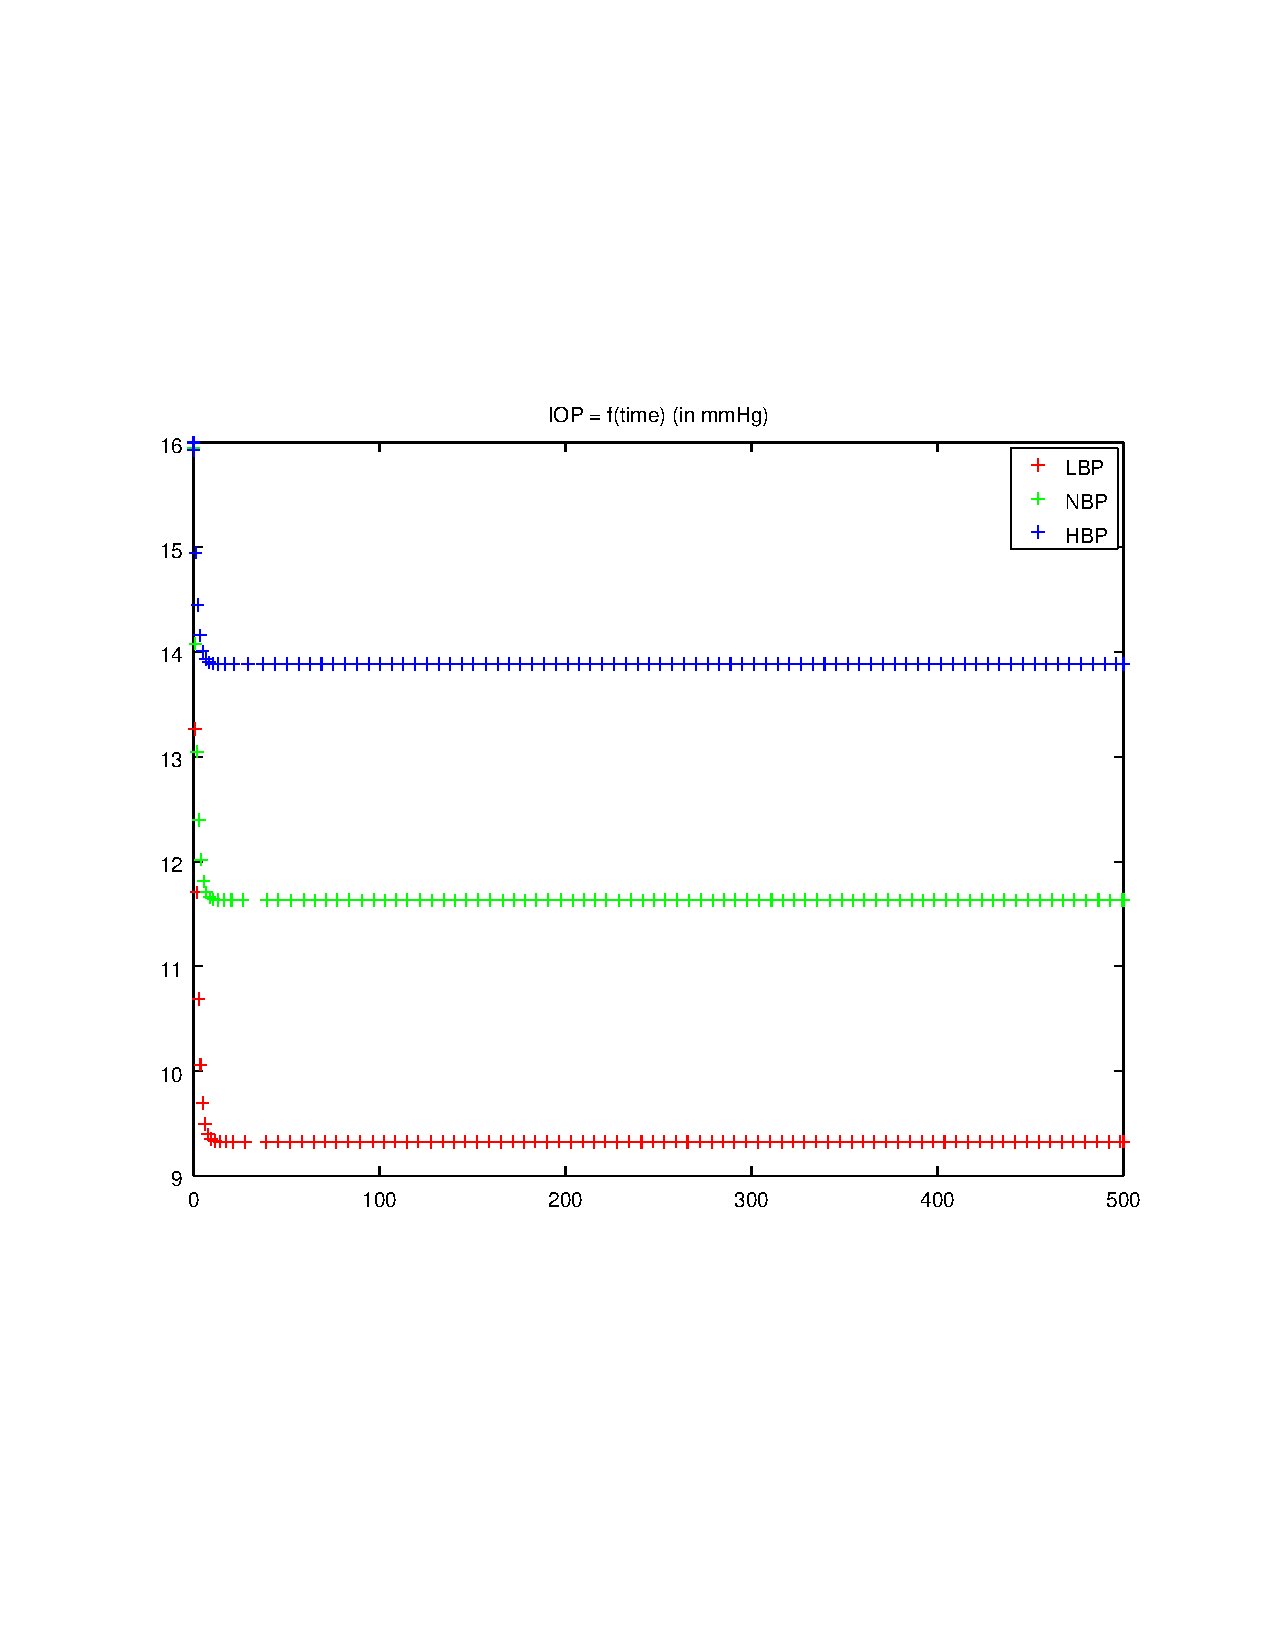
\includegraphics[width=0.45\textwidth]{images/IOP_time}
  }
  \subfigure[Time evolution of $C_2$\label{fig:C2t}]{
   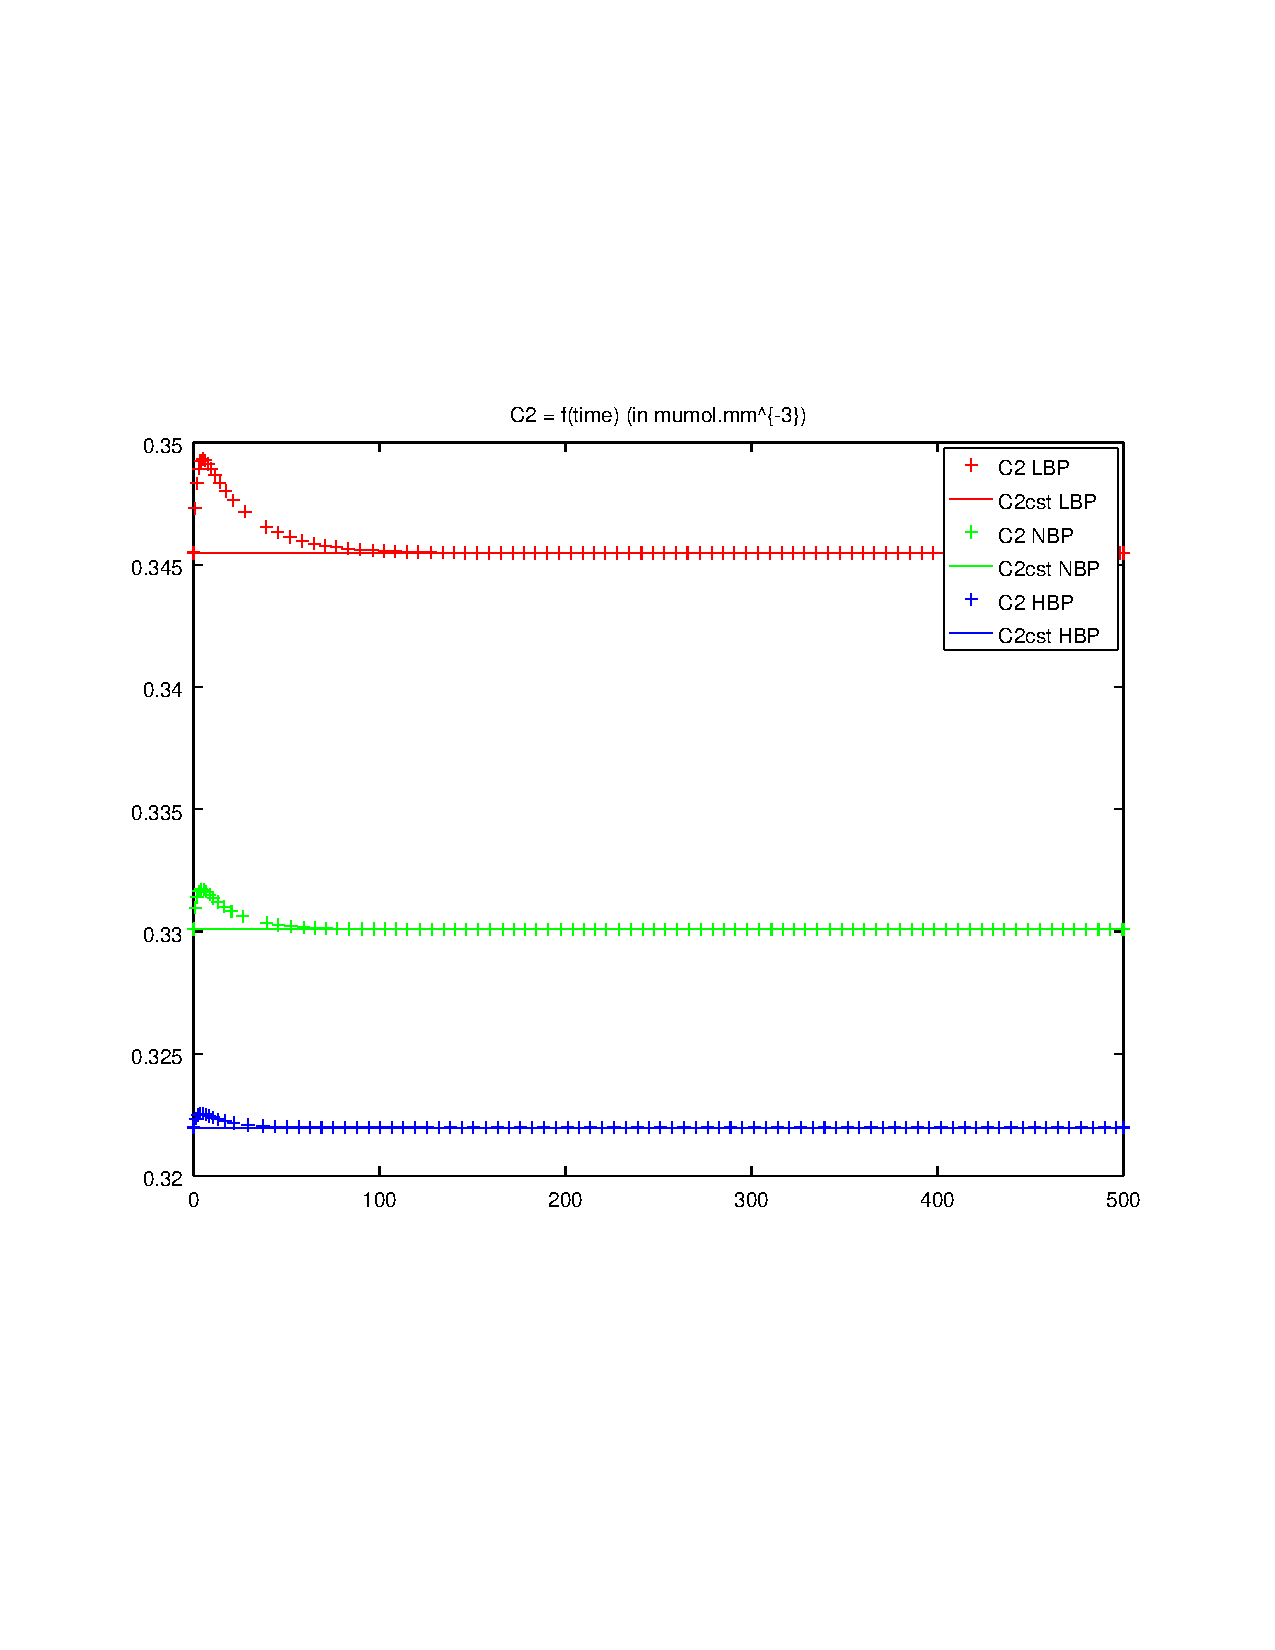
\includegraphics[width=0.45\textwidth]{images/C2_time}
 }
 
  \caption[text1]{Time evolution of IOP and $C_2$ }
    \label{fig:tevolpc2}
\end{figure}
%
\begin{figure}[h]


\begin{center}
  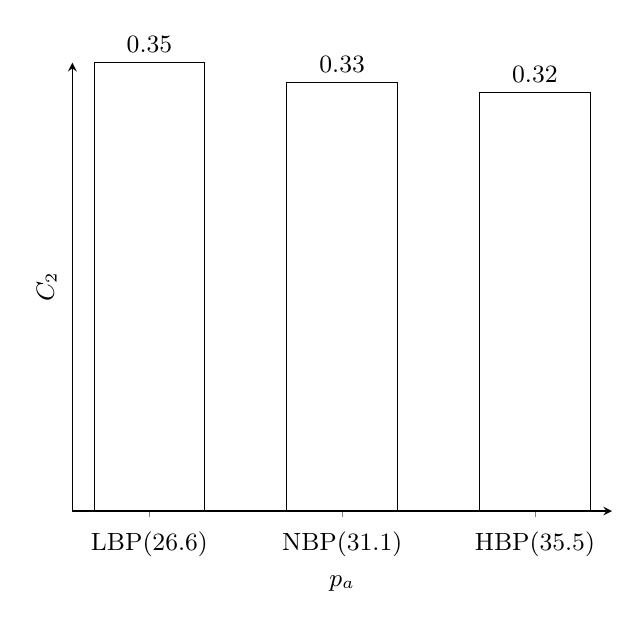
\begin{tikzpicture}[font=\small]
    \begin{axis}[
      ybar,
      bar width=40pt,
      xlabel={$p_a$},
      ylabel={$C_2$},
      ymin=0,
      ytick=\empty,
      xtick=data,
      axis x line=bottom,
      axis y line=left,
      enlarge x limits=0.2,
      %symbolic x coords={excellent,good,average,bad,awful},
      symbolic x coords = {LBP(26.6),NBP(31.1),HBP(35.5)},
      xticklabel style={anchor=base,yshift=-\baselineskip},
      nodes near coords={\pgfmathprintnumber\pgfplotspointmeta}
    ]
      \addplot[fill=white] coordinates {
        (LBP(26.6),0.345)
        (NBP(31.1),0.330)
        (HBP(35.5),0.322)
      };
    \end{axis}
  \end{tikzpicture}
  \end{center}

  \caption{$C_2 = f(p_a)$}
\end{figure}
\begin{figure}[h]
\begin{center}
  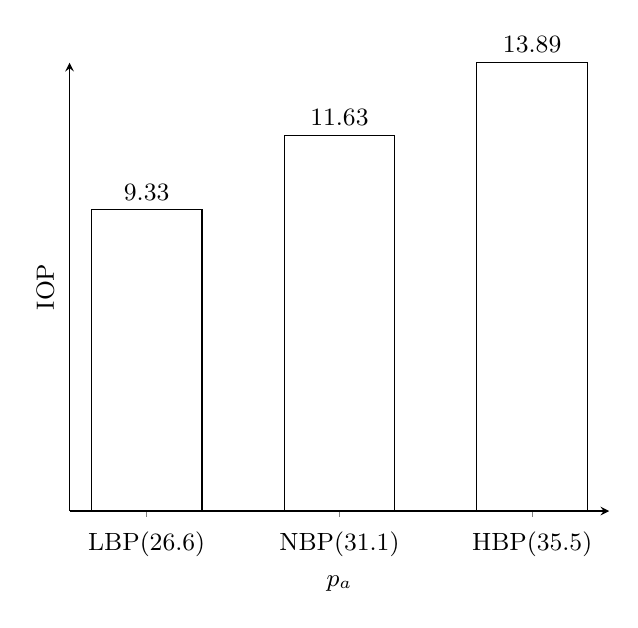
\begin{tikzpicture}[font=\small]
    \begin{axis}[
      ybar,
      bar width=40pt,
      xlabel={$p_a$},
      ylabel={IOP},
      ymin=0,
      ytick=\empty,
      xtick=data,
      axis x line=bottom,
      axis y line=left,
      enlarge x limits=0.2,
      %symbolic x coords={excellent,good,average,bad,awful},
      symbolic x coords = {LBP(26.6),NBP(31.1),HBP(35.5)},
      xticklabel style={anchor=base,yshift=-\baselineskip},
      nodes near coords={\pgfmathprintnumber\pgfplotspointmeta}
    ]
      \addplot[fill=white] coordinates {
        (LBP(26.6),9.3270)
        (NBP(31.1),11.632)
        (HBP(35.5),13.886)
      };
    \end{axis}
  \end{tikzpicture}
  \end{center}

  \caption{$IOP = f(p_a)$}
\end{figure}
\begin{figure}[h]
%\begin{tabular}{|l|l|l|l|}
%\hline
%BP (SBP/DBP)& LBP($100$/$70$)&NBP($120$/$80$) & HBP ($140$/$90$)\\
%$p_a$ (mmHg)& $p_a = 26.6$ & $p_a = 31.1$ & $p_a = 35.5$\\
%\hline
%IOP & $9.327$ & $11.632$ & $13.886$\\
%\hline
%\end{tabular}
\caption{table}
\end{figure}
\begin{figure}[h]
\begin{tabular}{|l|l|l|l|}
\hline
BP (SBP/DBP)& LBP($100$/$70$)&NBP($120$/$80$) & HBP ($140$/$90$)\\
$p_a$ (mmHg)& $p_a = 26.6$ & $p_a = 31.1$ & $p_a = 35.5$\\
\hline
$\Delta IOP$/$\Delta R $& $0.713$ & $1.022$ & $1.324$\\
\hline
\end{tabular}
\caption{Impact of $R$ on IOP}
\end{figure}
\begin{figure}[h]
\begin{tabular}{|l|l|l|l|}
\hline
BP (SBP/DBP)& LBP($100$/$70$)&NBP($120$/$80$) & HBP ($140$/$90$)\\
$p_a$ (mmHg)& $p_a = 26.6$ & $p_a = 31.1$ & $p_a = 35.5$\\
\hline
$\Delta IOP$/$\Delta L_p $& $13.072$ & $18.728$ & $24.261$\\
\hline
\end{tabular}
\caption{Impact of $L_p$ on IOP}
\end{figure}
